\documentclass{beamer}

%%%%%% PACKAGES %%%%%%
\usepackage[utf8x]{inputenc}
\usepackage[T1]{fontenc}
\usepackage[french]{babel}

\usepackage{datetime}
\selectlanguage{french}

\usepackage{hyperref}
\usepackage[numbers]{natbib}
\usepackage{array}
\usepackage{graphicx}
\usepackage{tikz}
\usetikzlibrary{snakes,arrows,shapes,calc}

%%%%%%%%%% CUSTOM COMMANDS %%%%%%%%%%

\newcommand{\okay}{
\includegraphics[height=0.5cm]{img/check.png}}
\newcommand{\nope}{
\includegraphics[height=0.5cm]{img/cross.png}}
\newcommand{\sortof}{
\includegraphics[width=0.5cm]{img/tilde.png}}

\newcommand{\ZZ}{\mathbb{Z}}
\newcommand{\Uu}{\mathcal{U}}

\newcommand{\la}{\leftarrow}
\newcommand{\ra}{\rightarrow}
\newcommand{\lra}{\leftrightarrow}

\newcommand{\Lla}{\longleftarrow}
\newcommand{\Lra}{\longrightarrow}
\newcommand{\Llra}{\longleftrightarrow}

\newcommand{\set}[1]{\left\{ #1 \right\}}


%%%%%%%% THEME %%%%%%%%
\usetheme[sectionpage=progressbar, progressbar=frametitle, block=fill]{metropolis}

%%%%%%% METADATA %%%%%%%
\title{Clavardage en groupe chiffré bout-en-bout}
\author{Simon Fernandez}
\date{\formatdate{28}{05}{2018}}


%%%%%%%%%%%%%%%%%%%%%%%%%%%
%%%%%%%%%% START %%%%%%%%%%
\begin{document}

\maketitle

\begin{frame}{Overview}
  \setcounter{tocdepth}{1}
	\tableofcontents
\end{frame}

\section{Clavardage en groupe?}
\begin{frame}{Propriétés du clavardage \emph{vs.} conversation en personne}
	\begin{tabular}{cc}
  	\begin{tabular}{c}
    	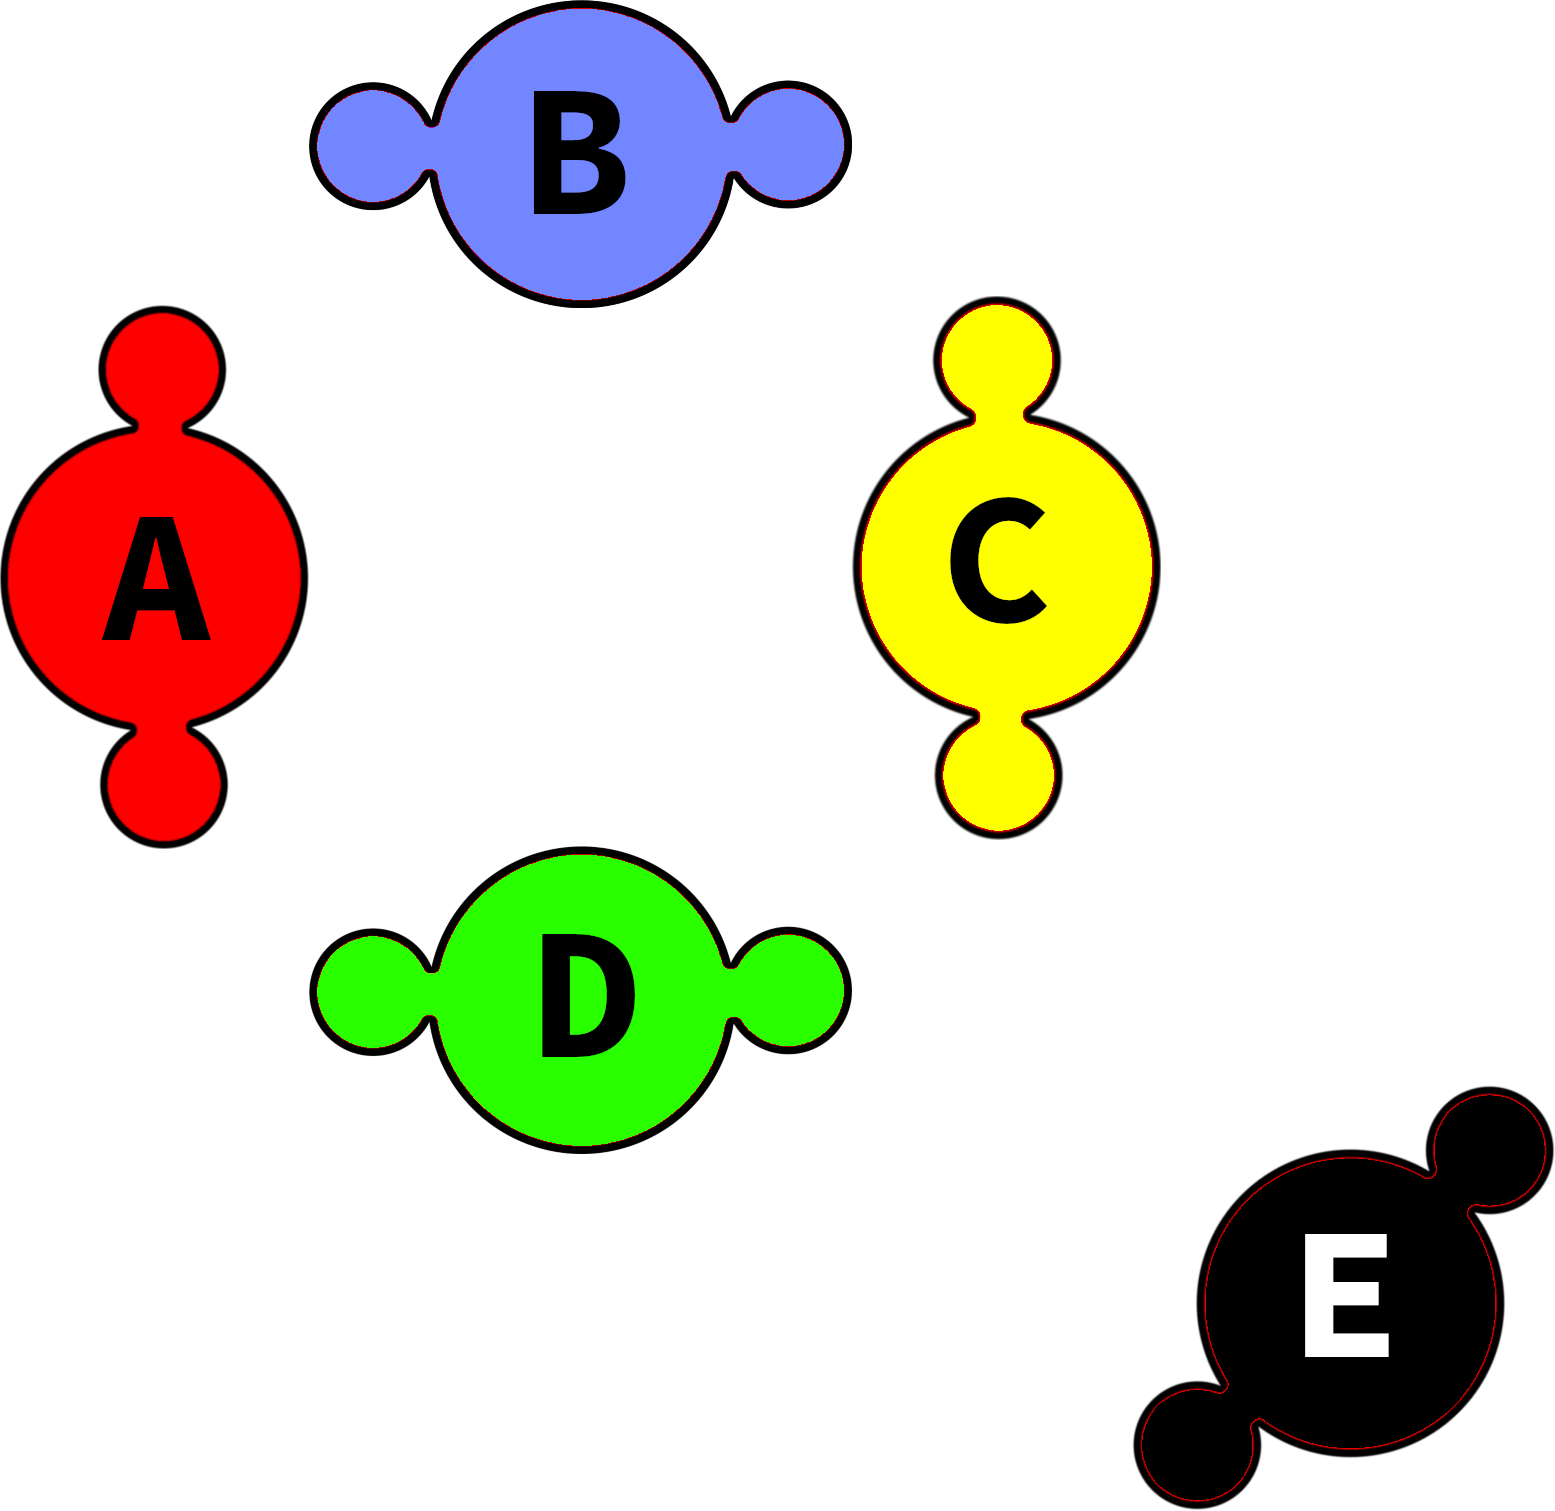
\includegraphics[height=5cm]{img/group_chat_eve.png}
  	\end{tabular}                   &

  	\begin{tabular}{c}
  		Authentification \\
  		\hline
  		Cohérence de participants \\
  		Cohérence de transcription \\
  		\hline
  		Répudiation de message \\
  		Répudiation de participation \\
  		\hline
  		Groupes dynamiques \\
  		\hline
  		Confidentialité persistente \\
  		Confidentialité rétroactive \\
  		Non-transitivité de paternité \\
  		\hline
  		Asynchrone
    \end{tabular}
	\end{tabular}
\end{frame}

\begin{frame}{Plus difficile que la configuration 1-1. Pourquoi?}
	\begin{tabular}{cc}
  	\begin{tabular}{c}
    	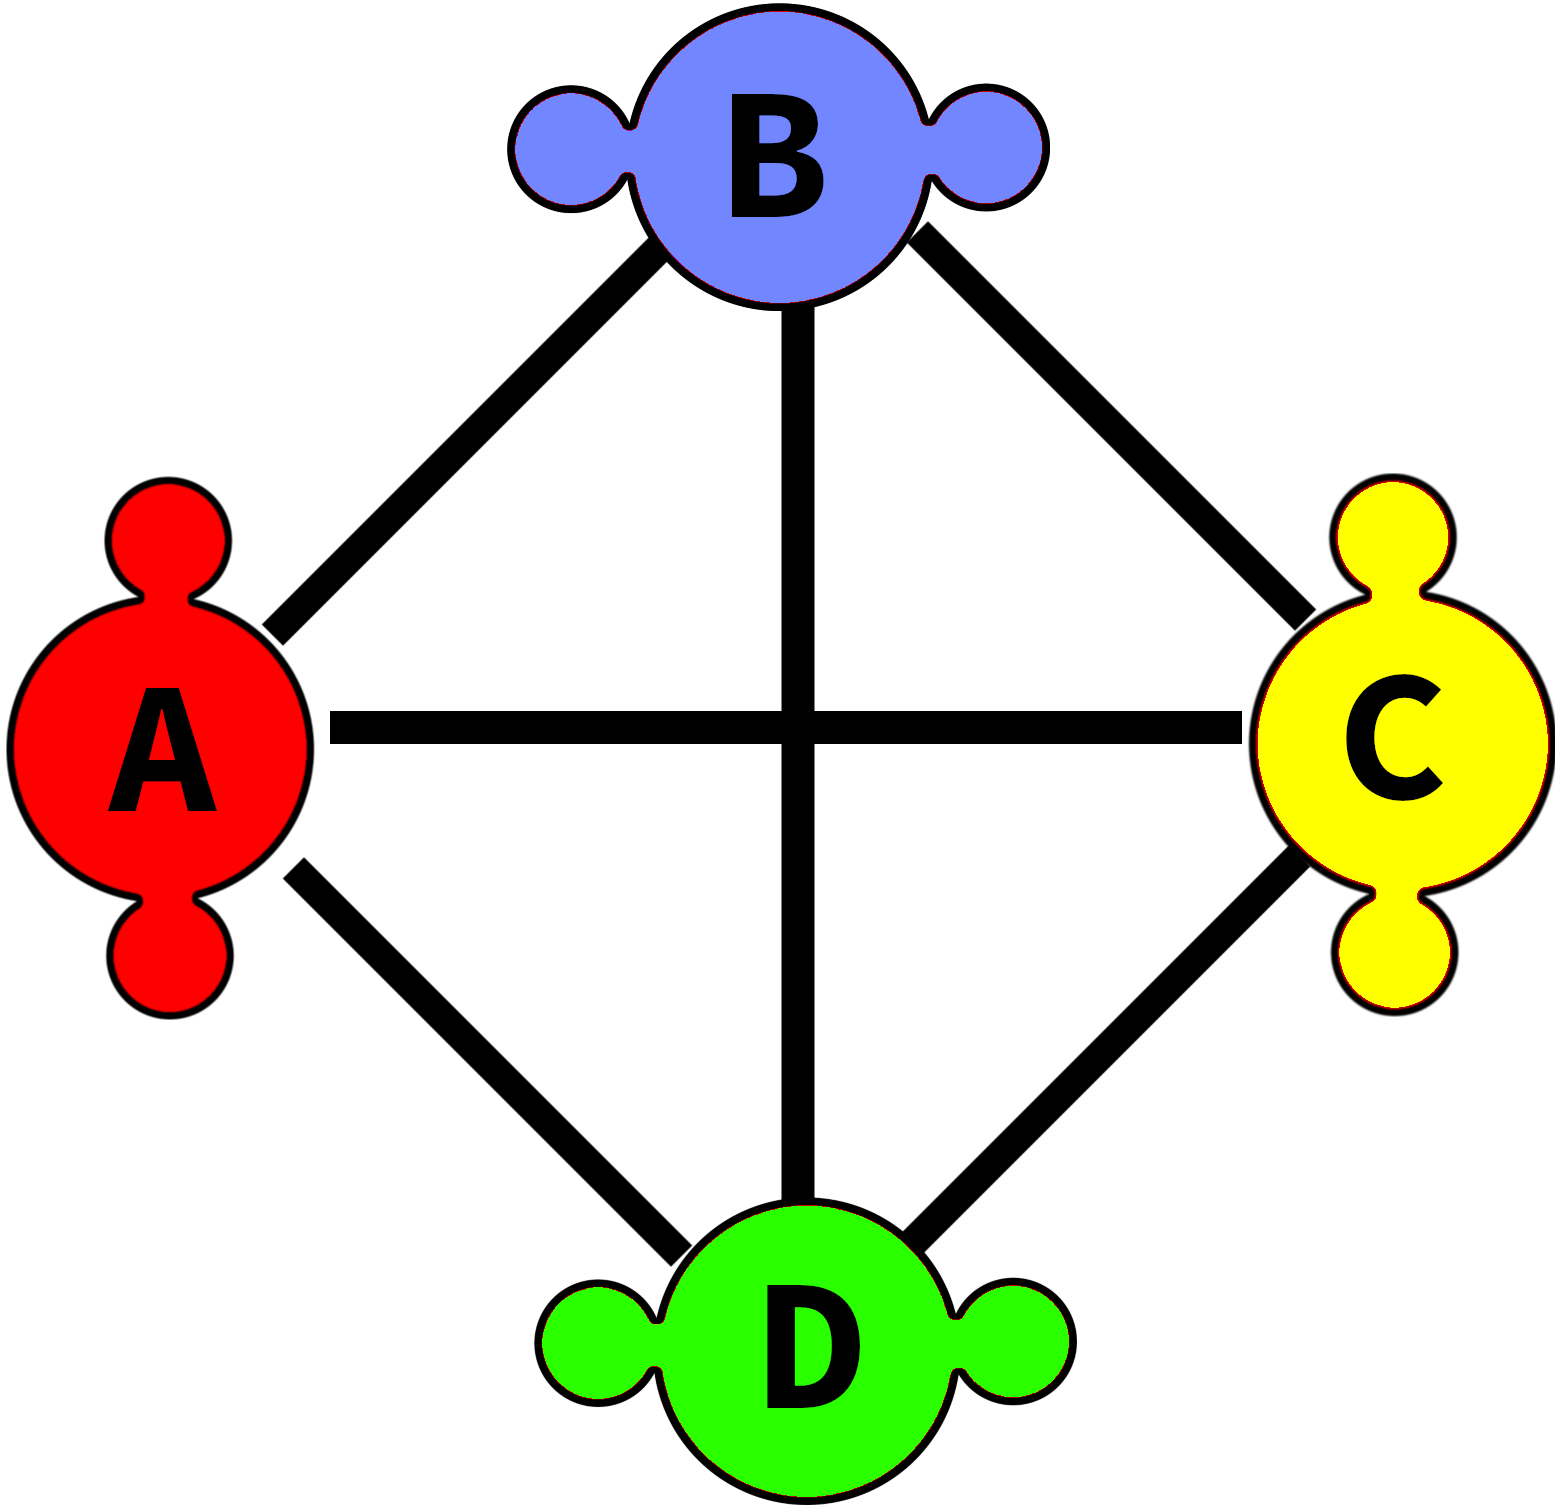
\includegraphics[height=5cm]{img/group_p2p.png}
  	\end{tabular}                   &

  	\begin{tabular}{c}
  		Cohérence de participants \\
  		Cohérence de transcription
    \end{tabular}
	\end{tabular}

\end{frame}


\section{mpOTR}
\begin{frame}{mpOTR -- Ian Goldberg et al. 2009~\cite{mpotr}}
	\begin{block}{Initialisation}
		\begin{itemize}
			\item Concensus sur une liste de participants;
      \item Échange de clef (EDC) en groupe;
			\item Déduction des clefs de chiffrement et de signature.
		\end{itemize}
  \end{block}

	\begin{block}{Communication}
		\begin{itemize}
			\item Signature de messages;
			\item Chiffrement de messages;
      \item Envoie par canal de diffusion.
		\end{itemize}
  \end{block}

	\begin{block}{Fermeture}
		\begin{itemize}
			\item Concensus sur la transcription de la conversation;
			\item Suppression des clefs.
		\end{itemize}
  \end{block}
\end{frame}

\begin{frame}{mpOTR}
	\center
  	\begin{tabular}{c|c}
			                              & mpOTR  \\
			\hline
  		Authentification              & \okay  \\
  		\hline
  		Cohérence de participants     & \okay  \\
  		Cohérence de transcription    & \okay  \\
  		\hline
  		Répudiation de message        & \okay  \\
  		Répudiation de participation  & \okay  \\
  		\hline
  		Groupes dynamiques            & \nope  \\
  		\hline
  		Confidentialité persistente   & \nope  \\
  		Confidentialité rétroactive   & \nope  \\
  		Non-transitivité de paternité & \nope  \\
  		\hline
  		Asynchrone                    & \sortof
    \end{tabular}
\end{frame}


\section{GOTR}
\begin{frame}{GOTR -- Liu et al.~\cite{gotr}}
	\center
	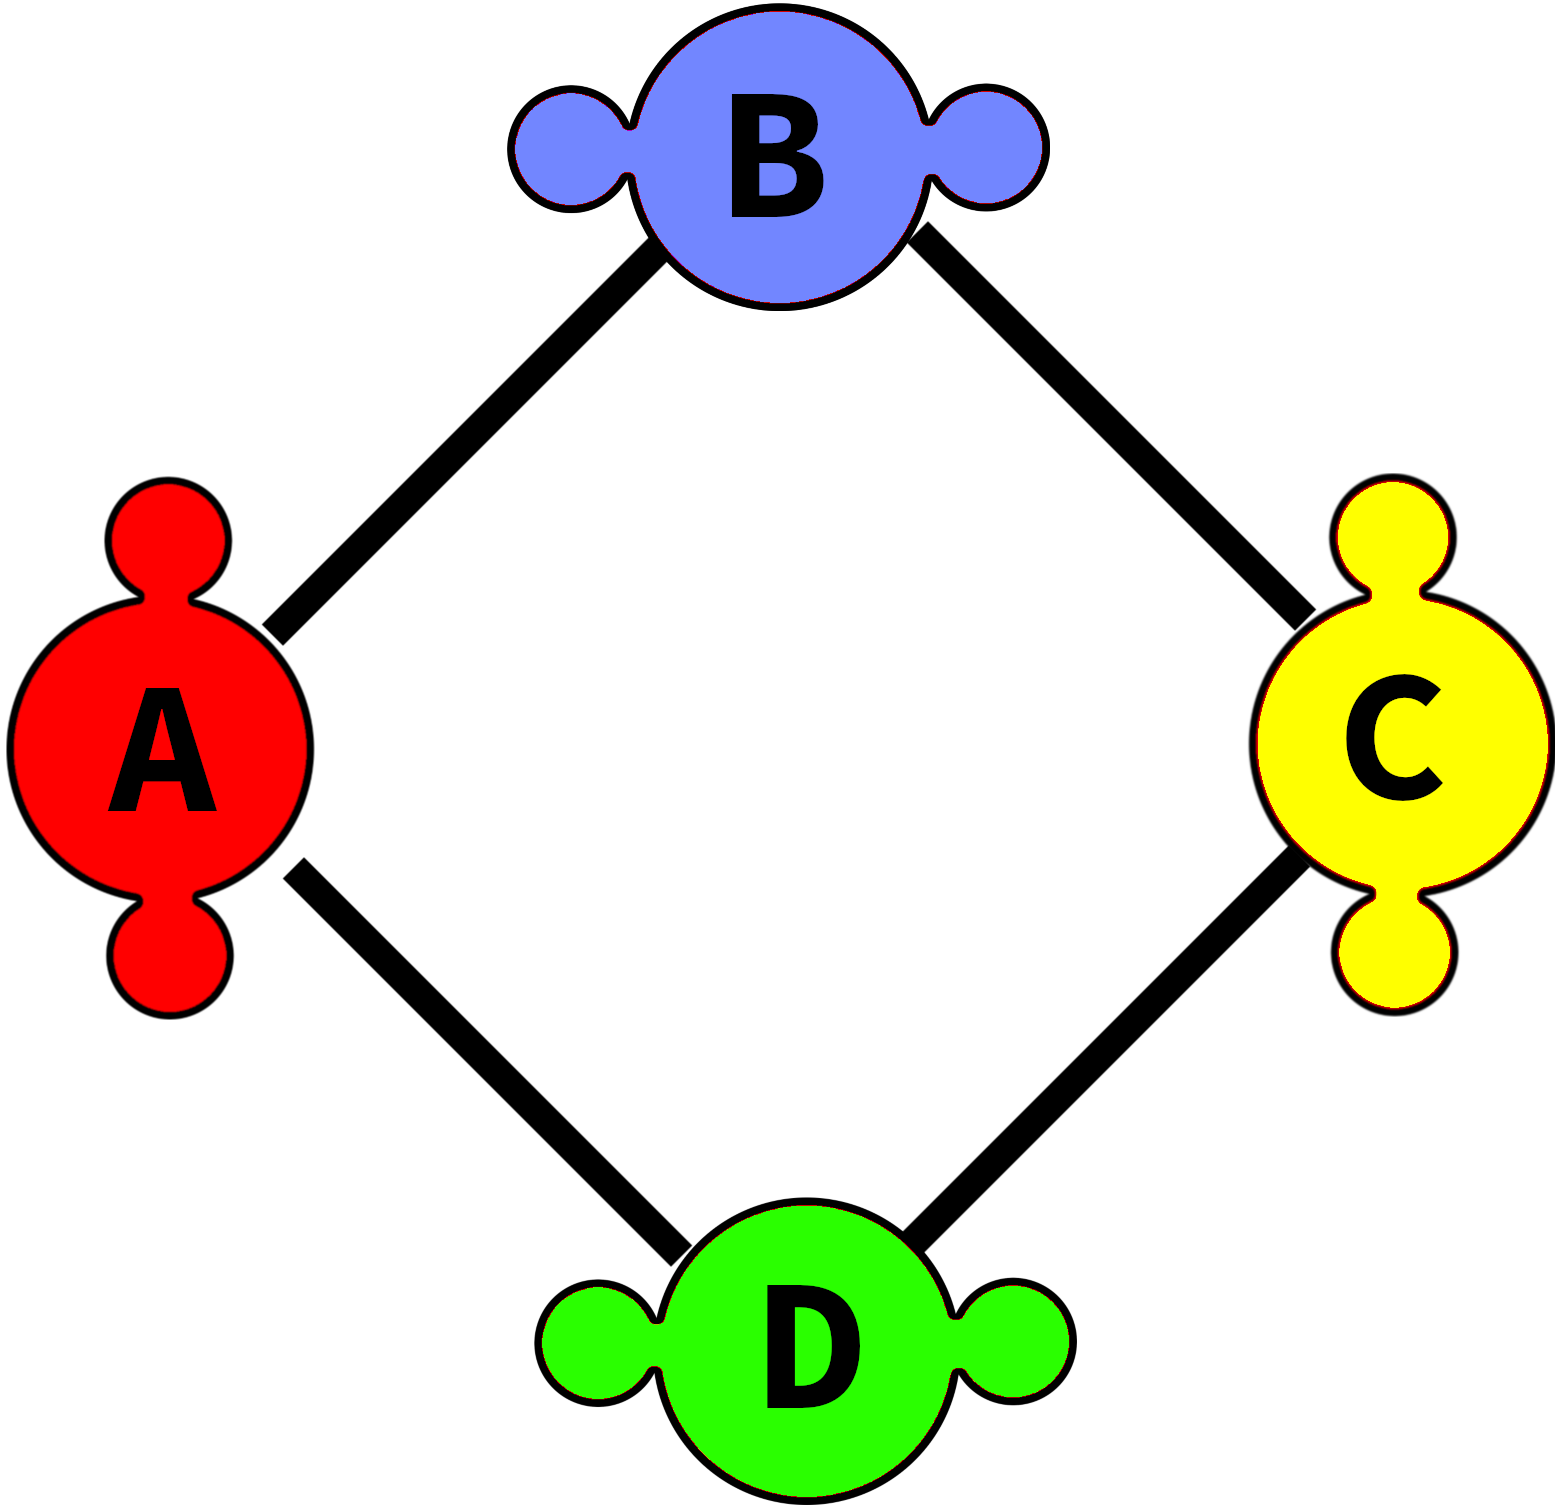
\includegraphics[height=6cm]{img/group_ring4.png}
\end{frame}

\begin{frame}{GOTR -- Liu et al.~\cite{gotr}}
	\center
	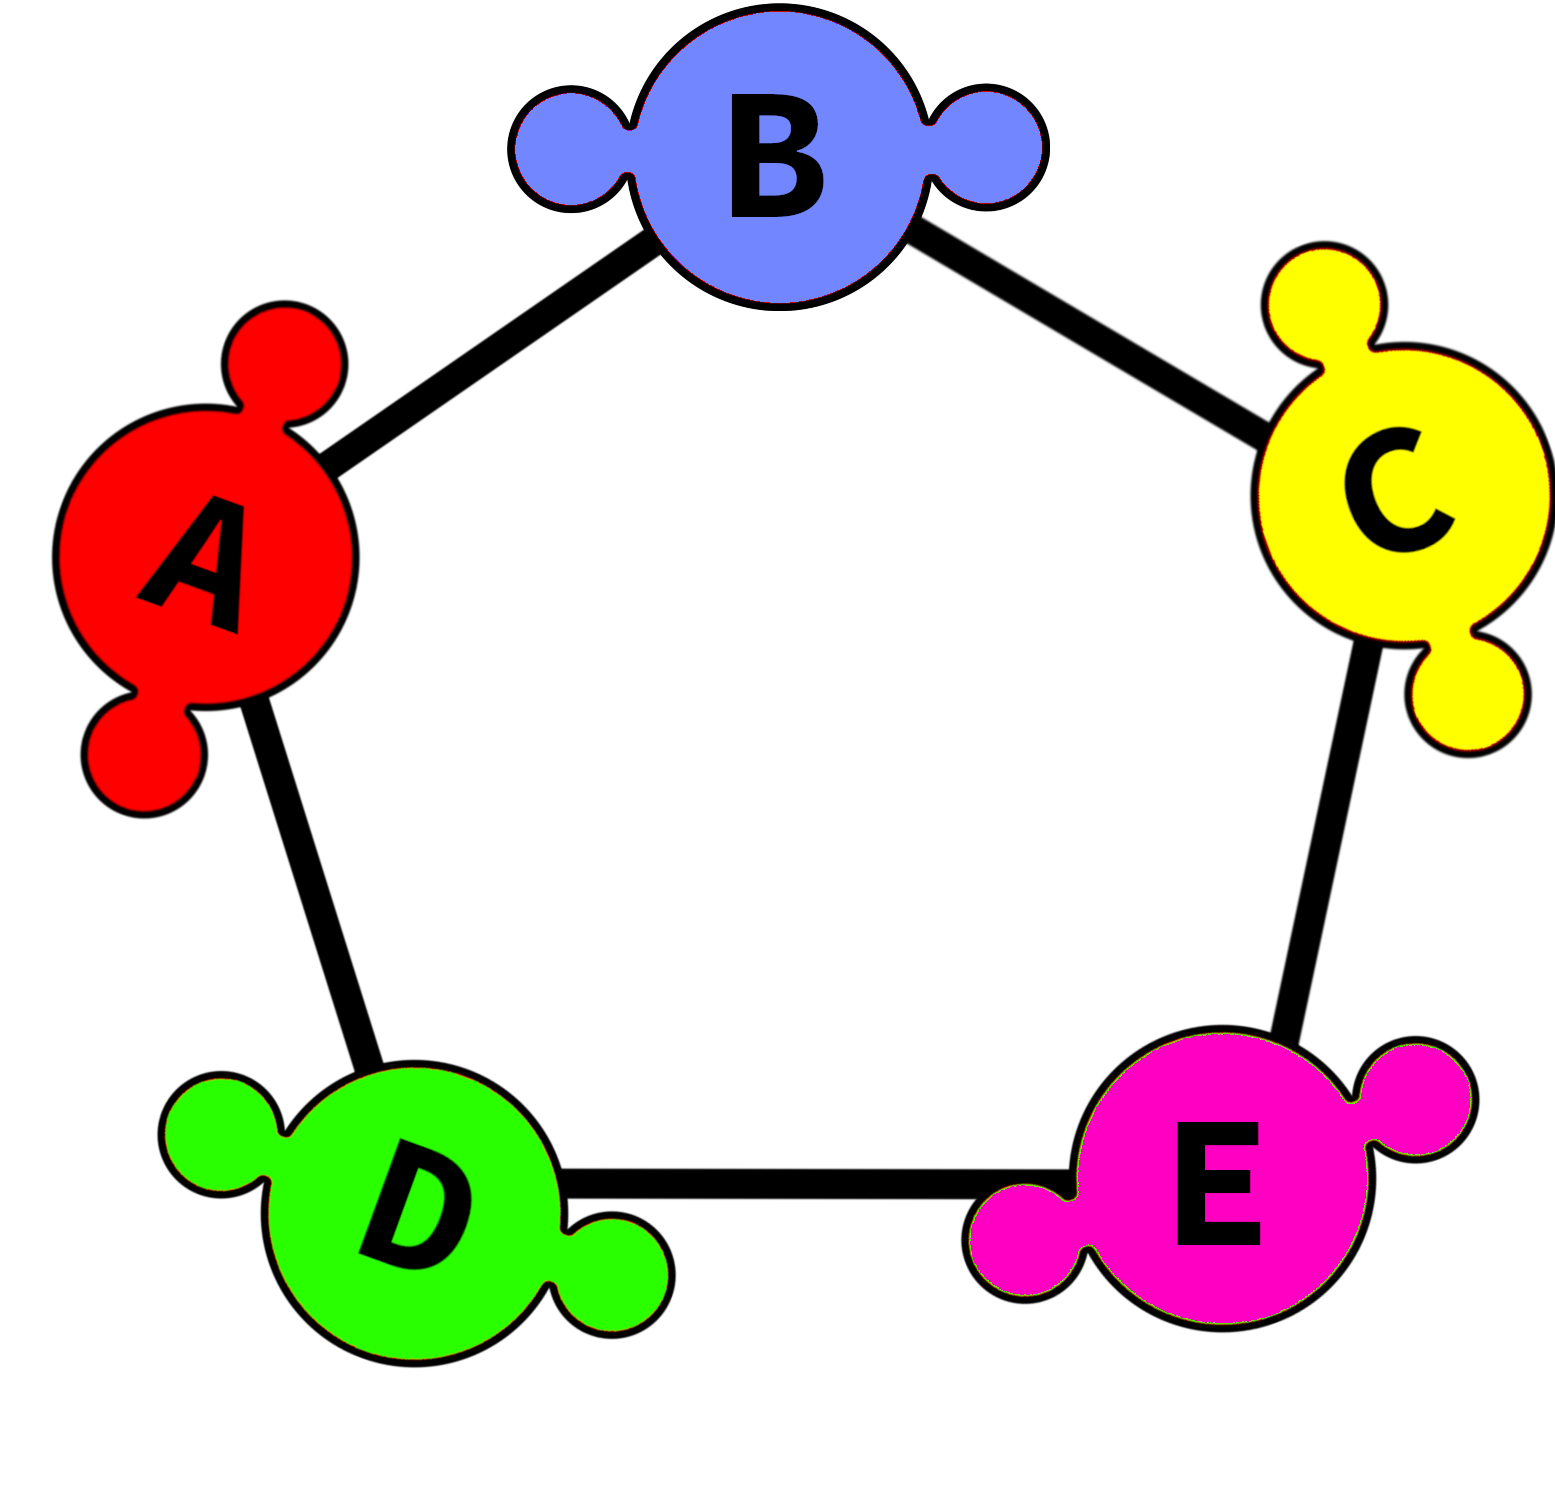
\includegraphics[height=6cm]{img/group_ring5.png}
\end{frame}

\begin{frame}{GOTR}

	\begin{block}{Mise à jour de clef}
		\begin{itemize}
      \item Génération des clefs (chiffrement et signature);
      \item Validation de la cohérence (individuel);
      \item Envoyer les nouvelles clefs (individuel);
			\item Déduction de la nouvelle clef de groupe.
		\end{itemize}
  \end{block}

	\begin{block}{Joindre/Se retirer}
		\begin{itemize}
			\item Ajouter au cercle;
			\item Appeler le protocole de mise à jour de clef.
		\end{itemize}
  \end{block}
\end{frame}

\begin{frame}{GOTR}
	\center
  	\begin{tabular}{c|cc}
			                              & mpOTR   & GOTR    \\
			\hline
  		Authentification              & \okay   & \okay   \\
  		\hline
  		Cohérence de participants     & \okay   & \okay   \\
  		Cohérence de transcription    & \okay   & \okay   \\
  		\hline
  		Répudiation de message        & \okay   & \okay   \\
  		Répudiation de participation  & \okay   & \okay   \\
  		\hline
  		Groupes dynamiques            & \nope   & \okay   \\
  		\hline
  		Confidentialité persistente   & \nope   & \sortof \\
  		Confidentialité rétroactive   & \nope   & \sortof \\
  		Non-transitivité de paternité & \nope   & \okay   \\
  		\hline
  		Asynchrone                    & \sortof & \nope
    \end{tabular}
\end{frame}

\section{Signal}
\begin{frame}{Étape technique: Diffie-Hellman}
	\center
	
\includegraphics[height=8cm]{img/stand-back-im-gonna-try-science.jpg}
\end{frame}

\begin{frame}{EDC Diffie-Hellman}
	\begin{block}{Groupe modulo}
		\begin{itemize}
			\item Cyclic Group $(G, \cdot)$ of prime order $p$
			\item $\forall g \in G, g^p = e_G, g^{(p+1)} = g$
			\item Let $g \in G\setminus \set{e_G}$. $\forall a \in G, \exists n \in \ZZ / p\ZZ, a = g^n$
		\end{itemize}
	\end{block}

	\pause

	\begin{block}{Protocole}
	$$
    \begin{array}{rl}
      A :       & x \la \Uu(\ZZ / q\ZZ) \\
      B :       & y \la \Uu(\ZZ / q\ZZ) \\
      A \ra B : & g^x                   \\
      B \ra A : & g^y                   \\
      A :       & S = (g^y)^x           \\
      B :       & S = (g^x)^y           
    \end{array}
   $$
	\end{block}

\end{frame}

\begin{frame}{Cliquet asymétrique DH}
  \only<1>{
    \begin{block}{Initialisation}
      Compléter un EDC Diffie-Hellman (EDCDH) avec le secret commun
      $$S_0 = g^{xy}$$
    \end{block}
  }

  \only<2>{
	\begin{block}{Communication}
  	$$
      \begin{array}{rl}
        A :       & x' \la \Uu(\ZZ / q\ZZ) \\
        A \ra B : & \set{M, g^{x'}}_{S_0} \\
        A :       & S_1 = (g^y)^{x'} \\
        B :       & S_1 = (g^{x'})^y \\
        B :       & y' \la \Uu(\ZZ / q \ZZ) \\
        B \ra A : & \set{M', g^{y'}}_{S_1} \\
        B :       & S_2 = (g^{x'})^{y'} \\
        A :       & S_2 = (g^{y'})^{x'} \\
      \end{array}
    $$
	\end{block}
  }
\end{frame}

\begin{frame}{Double cliquet}
	\center
	\begin{tabular}{rcl}
		Alice                           &         & Bob                       \\
		\hline
    $(x_0, g^{x_0})$                & $\Llra$ & $(y_0, g^{y_0})$          \\
		\hline
		$S_0$                           &         & $S_0$                     \\
		\hline
		$\set{M_0, g^{x_1}}_{S_0}$      & $\Lra$  &                           \\
		\hline
		$S_{0, 1} \la H(S_0)$           &         &                           \\
		\hline
		$\set{M_1, g^{x_1}}_{S_{0, 1}}$ & $\Lra$  &                           \\
		\hline
		$S_{0, 2} \la H(S_{0, 1})$      &         &                           \\
		\hline
		$\set{M_2, g^{x_1}}_{S_{0, 2}}$ & $\Lra$  &                           \\
		\hline
		                                &         & $S_1 \la (g^{x_1})^{y_0}$ \\
		\hline
		                                & $\Lla$  & $\set{M_3, g^{y_1}}_{S_1}$
	\end{tabular}
\end{frame}

\begin{frame}{Signal: extension naïve en groupe (graphe complet)}
	\center
	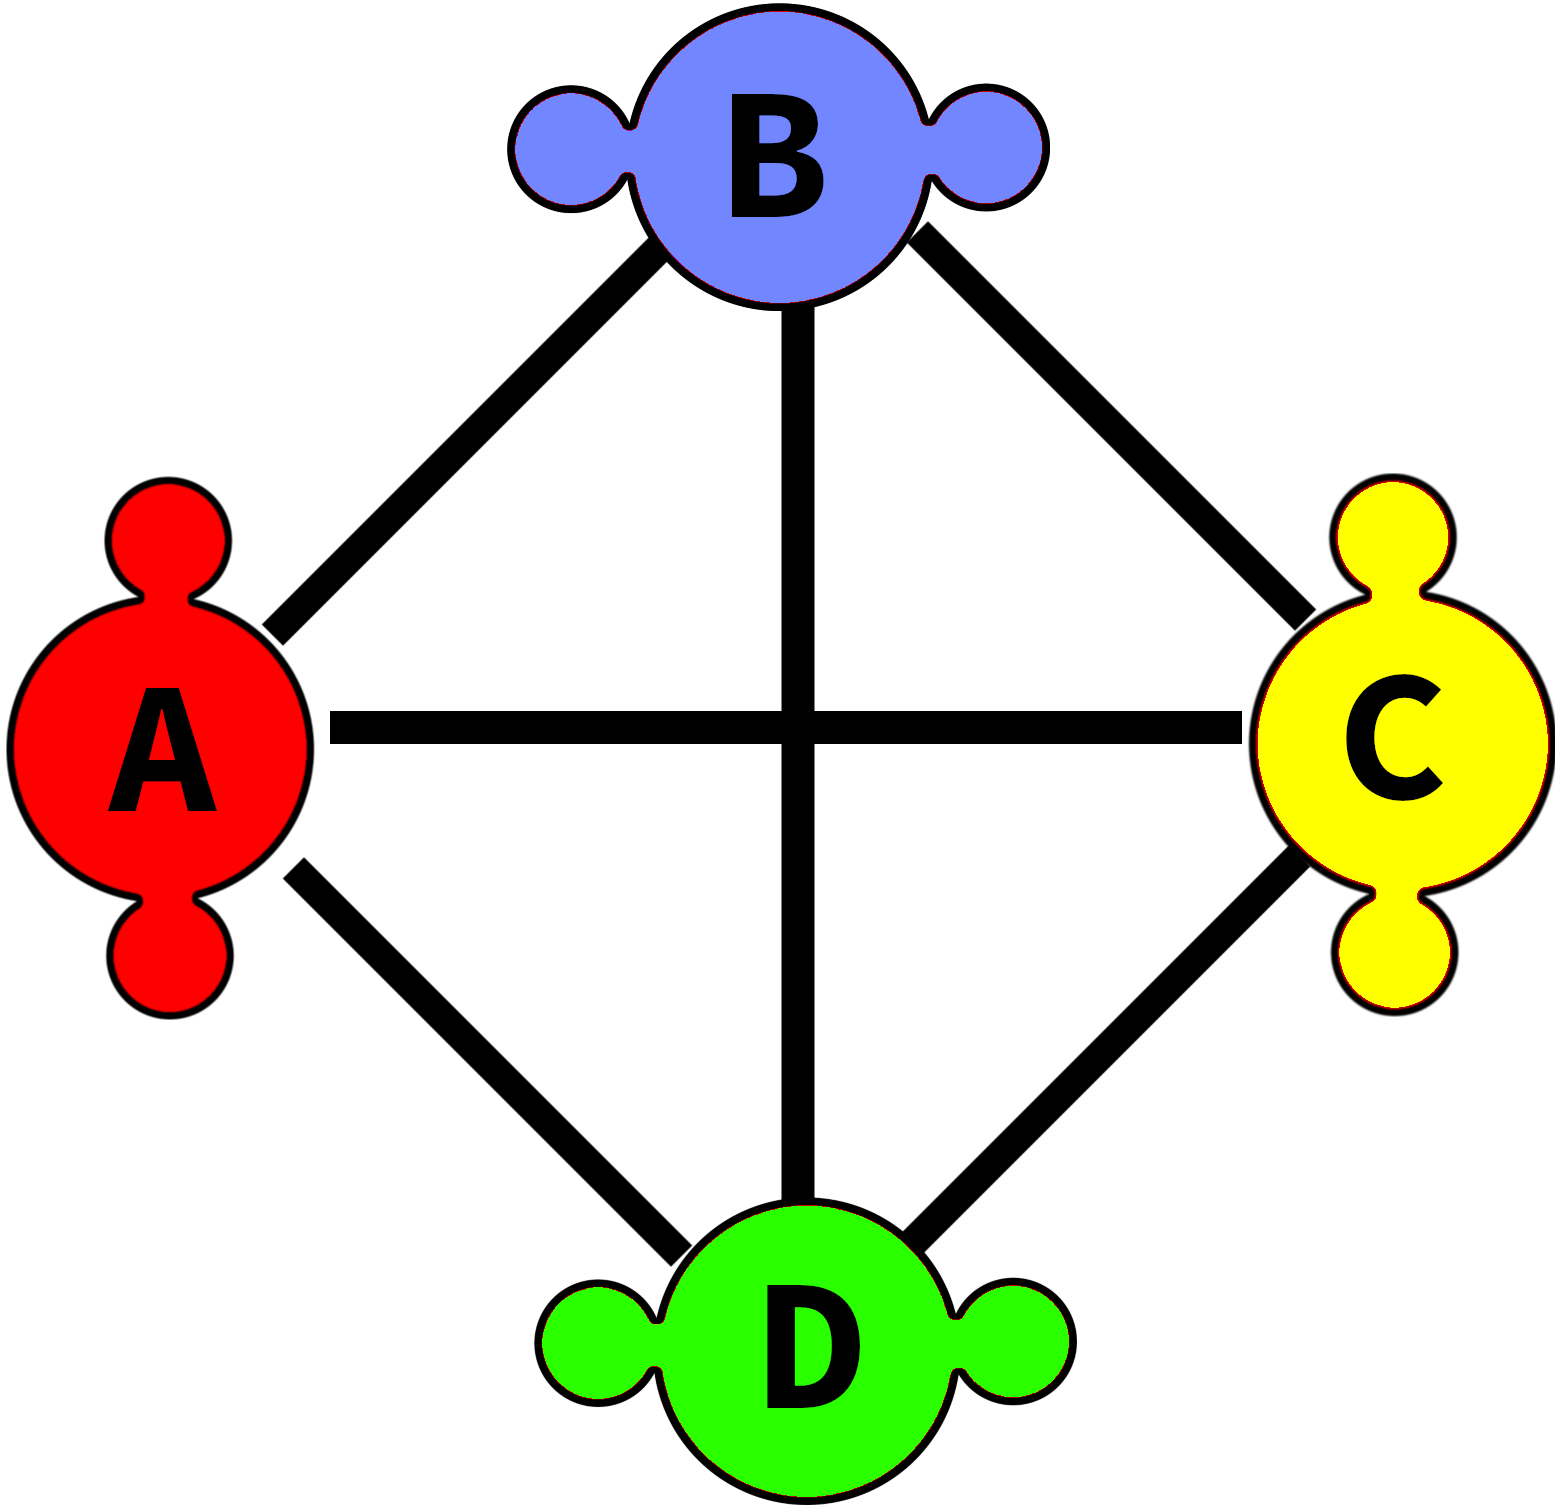
\includegraphics[height=6cm]{img/group_p2p.png}
\end{frame}

\begin{frame}{Signal}
	\center
  	\begin{tabular}{c|ccc}
			                              & mpOTR   & GOTR    & Signal  \\
			\hline
  		Authentification              & \okay   & \okay   & \okay   \\
  		\hline
  		Cohérence de participants     & \okay   & \okay   & \nope   \\
  		Cohérence de transcription    & \okay   & \okay   & \nope   \\
  		\hline
  		Répudiation de message        & \okay   & \okay   & \okay   \\
  		Répudiation de participation  & \okay   & \okay   & \okay   \\
  		\hline
  		Groupes dynamiques            & \nope   & \okay   & \okay   \\
  		\hline
  		Confidentialité persistente   & \nope   & \sortof & \sortof \\
  		Confidentialité rétroactive   & \nope   & \sortof & \okay   \\
  		Non-transitivité de paternité & \nope   & \okay   & \okay   \\
  		\hline
  		Asynchrone                    & \sortof & \nope   & \okay
    \end{tabular}
\end{frame}

\section{ART: Asynchronous Ratcheting Tree}

\begin{frame}{ART: Asynchronous Ratcheting Tree -- Cohn Gordon et al.~\cite{art}}
	\center
  \begin{tikzpicture}[]
		\path (3, 3) node[rectangle, draw](root) {$ tk: ABCD $}
  		(1, 2) node[rectangle, draw] (ab) {$AB$}
  		(5, 2) node[rectangle, draw] (cd) {$CD$}
  		(0, 1) node[rectangle, draw] (a) {$A$}
  		(2, 1) node[rectangle, draw] (b) {$B$}
  		(4, 1) node[rectangle, draw] (c) {$C$}
  		(6, 1) node[rectangle, draw] (d) {$D$};

		\draw[->] (ab) -- (root);
		\draw[->] (cd) -- (root);
		\draw[->] (a) -- (ab);
		\draw[->] (b) -- (ab);
		\draw[->] (c) -- (cd);
		\draw[->] (d) -- (cd);
	\end{tikzpicture}
\end{frame}

\begin{frame}{ART: Asynchronous Ratcheting Tree -- Cohn Gordon et al.~\cite{art}}
	\center
  \begin{tikzpicture}[]
		\path (3, 3) node[rectangle, draw](root) {$ tk = g^{x_{ab} x_{cd}} $}
  		(1, 2) node[rectangle, draw] (ab) {$x_{ab} = g^{x_a x_b}$}
  		(5, 2) node[rectangle, draw] (cd) {$x_{cd} = g^{x_c x_d}$}
  		(0, 1) node[rectangle, draw] (a) {$x_a$}
  		(2, 1) node[rectangle, draw] (b) {$x_b$}
  		(4, 1) node[rectangle, draw] (c) {$x_c$}
  		(6, 1) node[rectangle, draw] (d) {$x_d$};

		\draw[->] (ab) -- (root);
		\draw[->] (cd) -- (root);
		\draw[->] (a) -- (ab);
		\draw[->] (b) -- (ab);
		\draw[->] (c) -- (cd);
		\draw[->] (d) -- (cd);
	\end{tikzpicture}

	\center
  \begin{tikzpicture}[]
		\path (3, 3) node[rectangle, draw](root) {$ g^{tk} $}
  		(1, 2) node[rectangle, draw] (ab) {$g^{x_{ab}}$}
  		(5, 2) node[rectangle, draw] (cd) {$g^{x_{cd}}$}
  		(0, 1) node[rectangle, draw] (a) {$g^{x_a}$}
  		(2, 1) node[rectangle, draw] (b) {$g^{x_b}$}
  		(4, 1) node[rectangle, draw] (c) {$g^{x_c}$}
  		(6, 1) node[rectangle, draw] (d) {$g^{x_d}$};

		\draw[->] (ab) -- (root);
		\draw[->] (cd) -- (root);
		\draw[->] (a) -- (ab);
		\draw[->] (b) -- (ab);
		\draw[->] (c) -- (cd);
		\draw[->] (d) -- (cd);
	\end{tikzpicture}
\end{frame}

\begin{frame}{ART}
	\center
  \begin{tikzpicture}[]
  	\path (0,0) node(sk0){$sk_0$}
			(2, 1) node (tk0){$tk_1$}
  		(2, 0) node[rectangle, draw](kdf1){$KDF$}
  		(4, 0) node(sk1){$sk_1$}
			(6, 1) node (tk1){$tk_2$}
  		(6, 0) node[rectangle, draw](kdf2){$KDF$}
  		(8, 0) node(sk2){$sk_2$};

  	\draw[->](sk0) -- (kdf1);
		\draw[->](tk0) -- (kdf1);
		\draw[->](kdf1) -- (sk1);
  	\draw[->](sk1) -- (kdf2);
		\draw[->](tk1) -- (kdf2);
		\draw[->](kdf2) -- (sk2);
  \end{tikzpicture}

\end{frame}

\begin{frame}{ART : envoie de messages}
	\begin{block}{Envoie}
		\begin{itemize}
			\item Chiffrement avec $sk$;
      \item Envoie par canal de diffusion;
			\item Mise à jour de la clef.
		\end{itemize}
	\end{block}

	\begin{block}{Mise à jour de clef}
		\begin{itemize}
			\item Générer une nouvelle paire $x, g^x$;
      \item Diffuser les nouvelles clefs résultantes sur le chemin menant à sa feuille.
		\end{itemize}
	\end{block}
\end{frame}

\begin{frame}{ART : Mise à jour de clef}
	\center
  \begin{tikzpicture}[]
		\path (3, 3) node[rectangle, draw](root) {$ g^{tk} $}
  		(1, 2) node[rectangle, draw] (ab) {$g^{x_{ab}}$}
  		(5, 2) node[rectangle, draw] (cd) {$g^{x_{cd}}$}
  		(0, 1) node[rectangle, draw] (a) {$g^{x_a}$}
  		(2, 1) node[rectangle, draw] (b) {$g^{x_b}$}
  		(4, 1) node[rectangle, draw] (c) {$g^{x_c}$}
  		(6, 1) node[rectangle, draw] (d) {$g^{x_d}$};

		\draw[->] (ab) -- (root);
		\draw[->] (cd) -- (root);
		\draw[->] (a) -- (ab);
		\draw[->] (b) -- (ab);
		\draw[->] (c) -- (cd);
		\draw[->] (d) -- (cd);
	\end{tikzpicture}

  \begin{tikzpicture}[]
		\path (3, 3) node[rectangle, fill=red, draw](root) {$ tk' $}
  		(1, 2) node[rectangle, fill=red, draw] (ab) {$x_{ab}'$}
  		(5, 2) node[rectangle, draw] (cd) {$x_{cd}$}
  		(0, 1) node[rectangle, draw] (a) {$x_a$}
  		(2, 1) node[rectangle, fill=red, draw] (b) {$x_b'$}
  		(4, 1) node[rectangle, draw] (c) {$x_c$}
  		(6, 1) node[rectangle, draw] (d) {$x_d$};

		\draw[->] (ab) -- (root);
		\draw[->] (cd) -- (root);
		\draw[->] (a) -- (ab);
		\draw[->] (b) -- (ab);
		\draw[->] (c) -- (cd);
		\draw[->] (d) -- (cd);
	\end{tikzpicture}
\end{frame}

\begin{frame}{ART : Configuration}
	\begin{block}{Construction de l'arbre}
  	\begin{itemize}
  		\item Retrouver la clef signée de tous les participants;
			\item Diffuser les clefs publiques de chacun des membres aux autres;
			\item Diffuser la topologie de l'arbre;
			\item Commencer la conversation.
  	\end{itemize}
	\end{block}
\end{frame}

\begin{frame}{ART}
	\center
  	\begin{tabular}{c|cccc}
			                              & mpOTR   & GOTR    & Signal  & ART   \\
			\hline
  		Authentification              & \okay   & \okay   & \okay   & \nope \\
  		\hline
  		Cohérence de participants     & \okay   & \okay   & \nope   & \okay \\
  		Cohérence de transcription    & \okay   & \okay   & \nope   & \nope \\
  		\hline
  		Répudiation de message        & \okay   & \okay   & \okay   & \okay \\
  		Répudiation de participation  & \okay   & \okay   & \okay   & \okay \\
  		\hline
  		Groupes dynamiques            & \nope   & \okay   & \okay   & \okay \\
  		\hline
  		Confidentialité persistente   & \nope   & \sortof & \sortof & \okay \\
  		Confidentialité rétroactive   & \nope   & \sortof & \okay   & \okay \\
  		Non-transitivité de paternité & \nope   & \okay   & \okay   & \okay \\
  		\hline
  		Asynchrone                    & \sortof & \nope   & \okay   & \okay
    \end{tabular}
\end{frame}

\section{Et maintenant?}
\begin{frame}{ART 2.0 : avec authentification}
	\begin{block}{Idée principale}
		\begin{itemize}
			\item Clef publique unique;
			\item Clefs dynamiques.
		\end{itemize}
	\end{block}
	\pause
	\begin{block}{Clefs dynamiques}
		\begin{itemize}
			\item $(x, g^x) \ra (x', g^{x'})$
			\item $f, h$ sujet à $g^{f(x)} = h(g^x)$
		\end{itemize}
	\end{block}
\end{frame}

\begin{frame}{ART : Dérivation de clefs DH}
	\begin{block}{Première tentative de solution}
		\begin{itemize}
			\item $f : x \ra 2x$
			\item $h : y \ra y^2$
			\item $g^{2x} = (g^x)^2$
		\end{itemize}
	\end{block}
	\pause
	\begin{block}{Adaptation}
		\begin{itemize}
			\item $f : x \ra tk\cdot x$
			\item $h : y \ra y^{tk}$
			\item $g^{tk\cdot x} = (g^x)^{tk}$
		\end{itemize}
	\end{block}
\end{frame}

\begin{frame}{ART : Pas parfait}
	\begin{block}{Problèmes}
		\begin{itemize}
			\item Première étape?
			\item Forgeabilité de transcription de conversation impossible;
			\item Crypto faillible?
		\end{itemize}
	\end{block}
	\center
	Travail en cours.
\end{frame}
\section*{Merci ! Questions ?}

\begin{frame}
  \begin{small}

    \bibliographystyle{abbrv}
    \bibliography{slides}
	\end{small}
\end{frame}

\end{document}
